\secru{Вводный миниурок KiCad}

\cp{http://ru.wikibooks.org/wiki/KiCad/Миниурок}

Этот миниурок ознакомит Вас с основами использования системы KiCad. Он содержит
информацию о всех шагах создания простой печатной платы: от рисования
электрической схемы до печати готового рисунка платы. В ходе урока Вам будут
представлены различные возможности KiCad и предложены эффективные пути решения
различных задач.

Руководство пользователя, поставляемое вместе с KiCad, содержит значительно
больше информации, чем этот урок. Ознакомтесь с ним, чтобы узнать больше об
использовании программы.

В качестве примера взята несложная универсальная плата управления
скоростью вращения шпинделя сверлилки печатных плат,
питаемого постоянным током 9..48В:

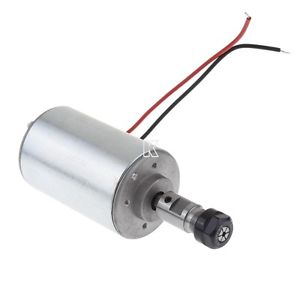
\includegraphics{SpindleDriver/spindle.jpeg}

Основным элементом схемы управления является дешевый и легко
доступный ШИМ-контроллер TL494CN в DIP-корпусе.



\secdown

\secru{Создание проекта}

Лучше всего для каждого проекта использовать раздельные папки; в противном
случае система может сбиться с толку, если файлы из разных проектов будут лежать
в одной папке. Проделайте следующие шаги:

\begin{enumerate}
  \item Создайте папку проекта \file{D:/ARM/SpindleDriver}
  \item Запустите программу KiCad
  \item Создайте проект (project)
  \begin{itemize}
    \item 
На панели инструментов KiCad выберите левую иконку с подсказкой\\
\menu{Начать новый проект}, используйте команду меню
\menu{Файл>Новый>Пустой} или сочетание клавиш \keys{Ctrl+N}.
    \item 
В диалоге \menu{Создать новый проект} выберите созданную папку
выберите только что созданную папку \file{D:/ARM/SpindleDriver} и
введите имя проекта \menu{\file{SpindleDriver}} и нажмите \menu{Сохранить}.
	\item
Если папка проекта содержит какие-то файлы, будет выведено окно выбора:
создать подпапку с именем проекта \menu{Yes}, или записать файл проекта
в указанную папку как есть \menu{No}. Нажмите No.
    \item 
Сохраните проект кнопкой \menu{Сохранить текущий проект}, \menu{Файл>Сохранить}
или \keys{Ctrl+S}.
	\item
В папке появится файл \file{SpindleDriver.pro}, содержащий установки вашего 
проекта. Файл имеет тектовый формат, поэтому при необходимости его можно открыть
в любом редакторе и вручную аккуратно подправить, например скорректировать
настройки зазоров печатной платы.
  \end{itemize}
\end{enumerate}

В правой части панели имеются четыре большие кнопки запуска компонентов KiCad.
Слева направо, это:

\begin{itemize}
\item EeSchema\ --- Редактор принципиальных схем
\item CvPcb\ --- Программа редактирования падстеков (отверстий и площадок)
\item Pcbnew\ --- Редактор печатных плат
\item GerbView\ --- Программа просмотра фотошаблонов в формате Gerber
\item Bitmap2Component\ --- Создание компонента из черно-белого изображения
(например логотипа)
\item PcbCalculator\ --- Калькулятор для печатных плат
\end{itemize}

Каждая кнопка запускает соответствующую программу. Мы будем использовать эти
программы по мере изучения.



\secup